\documentclass{utap}

\usepackage{wrapfig}
\usepackage{xepersian}

\graphicspath{{./img/}}

\title{تمرین شماره‌ی ۵}
\author{
	\href{mailto:bardia.eghbali@gmail.com??subject=[AP\%20S98\%20A5]\%20}{بردیا اقبالی},
	\href{mailto:seyedahmadpourihosseini@gmail.com?subject=[AP\%20S98\%20A5]\%20}{احمد پوری‌حسینی},
	\href{mailto:ahhabibvand@gmail.com?subject=[AP\%20S98\%20A5]\%20}{امیرحسین حبیب‌وند},
	\href{mailto:farzadhabibii98@gmail.com?subject=[AP\%20S98\%20A5]\%20}{فرزاد حبیبی}
}
\course{برنامه‌سازی پیشرفته}
\lecturer{رامتین خسروی}
\deadline{جمعه ۶ اردیبهشت ۱۳۹۸، ساعت ۲۳:۵۵}

\begin{document}
	\maketitle

	\section*{ سوپر ماریو }
مقدمه

برای مشاهده‌ی یک پیاده‌سازی کامل از بازی سوپر ماریو می‌توانید به \href{https://supermariobros.io/}{اینجا} 	مراجعه کنید. 
	\pagebreak

	\section{پیش‌تمرین}

در این پیش‌تمرین برنامه‌ای ساده را با کتاب‌خانۀ RSDL پیاده‌سازی می‌کنید تا بیشتر با آن آشنا شوید.


با کمک دستور draw\_img و استفاده از آرگومان src آن، می توانید تکه ای از یک تصویر را روی صفحه رسم کنید. در پوشه warmup تصویری از یک جدول 3x3 است که با اعداد 1 تا 9 پر شده. با استفاده از روش بالا برنامه ای بنویسید که به صورت تصادفی این جدول را به هم ریخته و روی صفحه رسم کند.

حالا می خواهیم با زدن دکمه R ترتیب خانه‌ها تغییر کند. برای این کار داخل یک حلقه با استفاده از تابع poll\_for\_event و get\_pressed\_key چک کنید که آیا دکمه‌ی R زده شده است یا نه. سپس مستطیل‌ها را دوباره محاسبه کنید و صفحه را بروزرسانی کنید.

تصویر زیر پنجره‌ی این برنامه را نشان می‌دهد.
	\begin{center}
		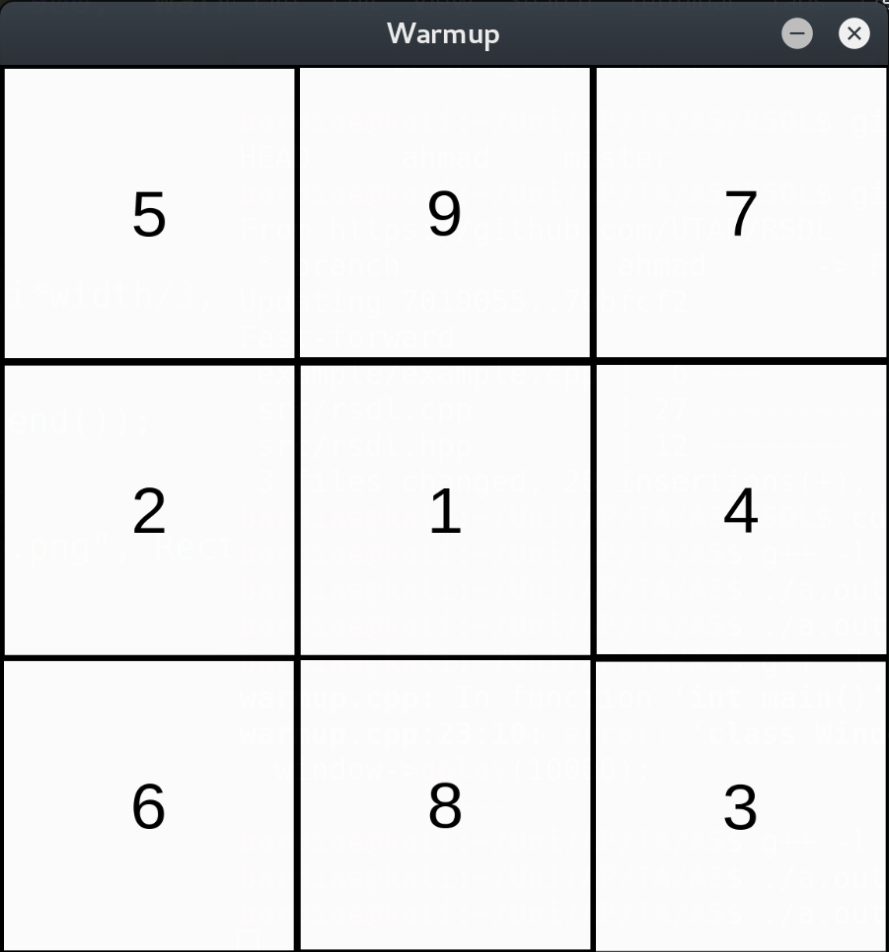
\includegraphics[width=8cm]{warmup.png}
	\end{center}
توجه کنید که این بخش برای آشنایی بیشتر شما با RSDL است و نیازی به تحویل آن نیست.
	\pagebreak

	\section{تمرین}
در این تمرین از شما انتظار می‌رود موارد زیر را پیاده‌سازی کنید و نکات گفته شده را رعایت کنید. تمرین از چند بخش مختلف تشکیل شده است که در ادامه به توضیح هر یک می‌پردازیم.

	\subsection{نقشه}
نقشه‌ی بازی به صورت یک جدول ۲ بعدی از کاراکترها به شما داده می‌شود. هر کاراکتر نشان‌دهنده‌ی محتوای یک خانه \LTRfootnote{tile} از نقشه‌ی بازی است. جدول زیر معنی هر کاراکتر را مشخص می‌کند.
	\begin{table}[H]
		\centering
		\begin{tabular}{ccc}
			\hline
			عنوان & کاراکتر معادل & تصویر\\
			\hline
			آجر‌ساده & b & تصویر\\
			\hline
			آجر شگفت انگیز دارای سکه & ? & تصویر\\
			\hline
			آجر شگفت انگیز دارای قارچ & m & تصویر\\
			\hline
			آجر شگفت انگیز دارای قارچ سلامتی & h & تصویر\\
			\hline
			بلوک معمولی & @ & تصویر\\
			\hline
			بلوک زمینی & \# & تصویر\\
			\hline
			ماریو & M & تصویر\\
			\hline
			گومبا کوچولو & l & تصویر\\
			\hline
			کوپا تروپا & k & تصویر\\
			\hline
			لوله  & | & تصویر\\
			\hline
			پرچم & f & تصویر\\
			\hline
		\end{tabular}
	\end{table}
عکس های مربوطه را می‌توانید در پوشه‌ی assets پیدا کنید. همچنین عکس پس‌زمینه‌ نیز داخل همین پوشه قرار دارد که باید پشت تمامی تصاویر دیگر رسم شود.

توجه کنید که پیاده‌سازی شما نباید به یک نقشه‌ی خاص برای بازی وابسته باشد، و باید بتواند با هر نقشه‌ی دلخواهی که مطابق فرمت گفته شده باشد، \textbf{بدون نیاز} به کامپایل مجدد، اجرا شود. به این  منظور برنامه‌ی شما باید آدرس نقشه‌ی مرحله‌ی مورد نظر را از خط‌فرمان\LTRfootnote{command line} دریافت کند. در هنگام تحویل پروژه، برنامه‌ی شما با یک نقشه‌ی جدید که قبلا ندیده‌اید تست خواهد شد.


\end{document}
